\documentclass{article}
\usepackage{fullpage,amssymb,amsmath,epsf}
\usepackage[12pt]{extsizes}
\usepackage{mathtools}
\usepackage{graphicx}
\usepackage{epstopdf}
\numberwithin{equation}{section}
\allowdisplaybreaks

\setlength{\textheight}{8in}

\usepackage[hang,flushmargin]{footmisc}

\newcommand\blfootnote[1]{%
	\begingroup
	\renewcommand\thefootnote{}\footnote{#1}%
	\addtocounter{footnote}{-1}%
	\endgroup
}

\pagestyle{myheadings}
\usepackage{graphicx}
\usepackage{subcaption}
%\renewcommand{\epsffile}[1]{
%	\includegraphics[width=\epsfxsize]{#1}
%}

\newcommand{\di}{{d}}
\newcommand{\nexp}{{n}}
\newcommand{\vcd}{{\textbf{D}}}


\documentclass{article}
\usepackage[top = 1.0in]{geometry}

\usepackage{graphicx}

\usepackage[utf8]{inputenc}
\usepackage{listings}
\usepackage[dvipsnames]{xcolor}
\usepackage{bm}
\usepackage{algorithm}
\usepackage{algpseudocode}
\usepackage{framed}

\definecolor{codegreen}{rgb}{0,0.6,0}
\definecolor{codegray}{rgb}{0.5,0.5,0.5}
\definecolor{codepurple}{rgb}{0.58,0,0.82}
\definecolor{backcolour}{rgb}{0.95,0.95,0.92}

\lstdefinestyle{mystyle}{
    backgroundcolor=\color{backcolour},   
    commentstyle=\color{codegreen},
    keywordstyle=\color{magenta},
    stringstyle=\color{codepurple},
    basicstyle=\ttfamily\footnotesize,
    breakatwhitespace=false,         
    breaklines=true,                 
    captionpos=b,                    
    keepspaces=true,                 
    numbersep=5pt,                  
    showspaces=false,                
    showstringspaces=false,
    showtabs=false,                  
    tabsize=2
}

\lstset{style=mystyle}

\newcommand{\di}{{d}}
\newcommand{\nexp}{{n}}
\newcommand{\nf}{{p}}
\newcommand{\vcd}{{\textbf{D}}}
\newcommand{\Int}{\mathbb{Z}}
\newcommand\bb{\ensuremath{\mathbf{b}}}
\newcommand\bs{\ensuremath{\mathbf{s}}}
\newcommand\bp{\ensuremath{\mathbf{p}}}
\newcommand{\relu} { \operatorname{ReLU} }
\newcommand{\smx} { \operatorname{softmax} }
\newcommand\bx{\ensuremath{\mathbf{x}}}
\newcommand\bh{\ensuremath{\mathbf{h}}}
\newcommand\bc{\ensuremath{\mathbf{c}}}
\newcommand\bW{\ensuremath{\mathbf{W}}}
\newcommand\by{\ensuremath{\mathbf{y}}}
\newcommand\bo{\ensuremath{\mathbf{o}}}
\newcommand\be{\ensuremath{\mathbf{e}}}
\newcommand\ba{\ensuremath{\mathbf{a}}}
\newcommand\bu{\ensuremath{\mathbf{u}}}
\newcommand\bv{\ensuremath{\mathbf{v}}}
\newcommand\bP{\ensuremath{\mathbf{P}}}
\newcommand\bg{\ensuremath{\mathbf{g}}}
\newcommand\bX{\ensuremath{\mathbf{X}}}
% real numbers R symbol
\newcommand{\Real}{\mathbb{R}}

% encoder hidden
\newcommand{\henc}{\bh^{\text{enc}}}
\newcommand{\hencfw}[1]{\overrightarrow{\henc_{#1}}}
\newcommand{\hencbw}[1]{\overleftarrow{\henc_{#1}}}

% encoder cell
\newcommand{\cenc}{\bc^{\text{enc}}}
\newcommand{\cencfw}[1]{\overrightarrow{\cenc_{#1}}}
\newcommand{\cencbw}[1]{\overleftarrow{\cenc_{#1}}}

% decoder hidden
\newcommand{\hdec}{\bh^{\text{dec}}}

% decoder cell
\newcommand{\cdec}{\bc^{\text{dec}}}

\usepackage[hyperfootnotes=false]{hyperref}
\hypersetup{
  colorlinks=true,
  linkcolor = blue,
  urlcolor  = blue,
  citecolor = blue,
  anchorcolor = blue,
  pdfborderstyle={/S/U/W 1}
}
\usepackage{nccmath}
\usepackage{mathtools}
\usepackage{graphicx,caption}
\usepackage[shortlabels]{enumitem}
\usepackage{epstopdf,subcaption}
\usepackage{psfrag}
\usepackage{amsmath,amssymb,epsf}
\usepackage{verbatim}
\usepackage{cancel}
\usepackage{color,soul}
\usepackage{bbm}
\usepackage{listings}
\usepackage{setspace}
\usepackage{float}
\definecolor{Code}{rgb}{0,0,0}
\definecolor{Decorators}{rgb}{0.5,0.5,0.5}
\definecolor{Numbers}{rgb}{0.5,0,0}
\definecolor{MatchingBrackets}{rgb}{0.25,0.5,0.5}
\definecolor{Keywords}{rgb}{0,0,1}
\definecolor{self}{rgb}{0,0,0}
\definecolor{Strings}{rgb}{0,0.63,0}
\definecolor{Comments}{rgb}{0,0.63,1}
\definecolor{Backquotes}{rgb}{0,0,0}
\definecolor{Classname}{rgb}{0,0,0}
\definecolor{FunctionName}{rgb}{0,0,0}
\definecolor{Operators}{rgb}{0,0,0}
\definecolor{Background}{rgb}{0.98,0.98,0.98}
\lstdefinelanguage{Python}{
    numbers=left,
    numberstyle=\footnotesize,
    numbersep=1em,
    xleftmargin=1em,
    framextopmargin=2em,
    framexbottommargin=2em,
    showspaces=false,
    showtabs=false,
    showstringspaces=false,
    frame=l,
    tabsize=4,
    % Basic
    basicstyle=\ttfamily\footnotesize\setstretch{1},
    backgroundcolor=\color{Background},
    % Comments
    commentstyle=\color{Comments}\slshape,
    % Strings
    stringstyle=\color{Strings},
    morecomment=[s][\color{Strings}]{"""}{"""},
    morecomment=[s][\color{Strings}]{'''}{'''},
    % keywords
    morekeywords={import,from,class,def,for,while,if,is,in,elif,else,not,and,or
    ,print,break,continue,return,True,False,None,access,as,,del,except,exec
    ,finally,global,import,lambda,pass,print,raise,try,assert},
    keywordstyle={\color{Keywords}\bfseries},
    % additional keywords
    morekeywords={[2]@invariant},
    keywordstyle={[2]\color{Decorators}\slshape},
    emph={self},
    emphstyle={\color{self}\slshape},
%
}
\lstMakeShortInline|

\pagestyle{empty} \addtolength{\textwidth}{1.0in}
\addtolength{\textheight}{0.5in}
\addtolength{\oddsidemargin}{-0.5in}
\addtolength{\evensidemargin}{-0.5in}
\newcommand{\ruleskip}{\bigskip\hrule\bigskip}
\newcommand{\nodify}[1]{{\sc #1}}
\newenvironment{answer}{\sf \begingroup\color{ForestGreen}}{\endgroup}%

\setlist[itemize]{itemsep=2pt, topsep=0pt}
\setlist[enumerate]{itemsep=6pt, topsep=0pt}

\setlength{\parindent}{0pt}
\setlength{\parskip}{4pt}
\setlist[enumerate]{parsep=4pt}
\setlength{\unitlength}{1cm}

\renewcommand{\Re}{{\mathbb R}}
\newcommand{\R}{\mathbb{R}}
\newcommand{\what}[1]{\widehat{#1}}

\renewcommand{\comment}[1]{}
\newcommand{\mc}[1]{\mathcal{#1}}
\newcommand{\half}{\frac{1}{2}}

\DeclareMathOperator*{\argmin}{arg\,min}

\def\KL{D_{KL}}
\def\xsi{x^{(i)}}
\def\ysi{y^{(i)}}
\def\zsi{z^{(i)}}
\def\E{\mathbb{E}}
\def\calN{\mathcal{N}}
\def\calD{\mathcal{D}}
\def\slack{\url{http://xcs229-scpd.slack.com/}}
\def\zipscriptalt{\texttt{python zip\_submission.py}}
\DeclarePairedDelimiter\abs{\lvert}{\rvert}%
 
\usepackage{bbding}
\usepackage{pifont}
\usepackage{wasysym}
\usepackage{amssymb}
\usepackage{framed}
\usepackage{scrextend}

\newcommand{\alns}[1] {
	\begin{align*} #1 \end{align*}
}

\newcommand{\pd}[2] {
 \frac{\partial #1}{\partial #2}
}
\renewcommand{\Re} { \mathbb{R} }
\newcommand{\btx} { \mathbf{\tilde{x}} }
\newcommand{\bth} { \mathbf{\tilde{h}} }
\newcommand{\sigmoid} { \operatorname{\sigma} }
\newcommand{\CE} { \operatorname{CE} }
\newcommand{\byt} { \hat{\by} }
\newcommand{\yt} { \hat{y} }

\newcommand{\oft}[1]{^{(#1)}}
\newcommand{\fone}{\ensuremath{F_1}}

\newcommand{\ac}[1]{ {\color{red} \textbf{AC:} #1} }
\newcommand{\ner}[1]{\textbf{\color{blue} #1}}
\begin{document}
\title{XCS229 Lecture Notes}
\author{Andrew Ng}
\date{}
\maketitle

\part*{Deep Learning}\blfootnote{Scribe: Albert Haque}

\noindent We now begin our study of deep learning. In this set of notes, we give an overview of neural networks, discuss vectorization and discuss training neural networks with backpropagation. 

\section{Neural Networks}

We will start small and slowly build up a neural network, step by step. Recall the housing price prediction problem from before: given the size of the house, we want to predict the price.

Previously, we fitted a straight line to the graph. Now, instead of fitting a straight line, we wish prevent negative housing prices by setting the absolute minimum price as zero. This produces a ``kink" in the graph as shown in Figure \ref{fig:housing}.

Our goal is to input some input $x$ into a function $f(x)$ that outputs the price of the house $y$. Formally, $f: x \rightarrow y$. One of the simplest possible neural networks is to define $f(x)$ as a single ``neuron" in the network where $f(x) = \max(ax + b, 0)$, for some coefficients $a,b$. What $f(x)$ does is return a single value: $(ax + b)$ or zero, whichever is greater. In the context of neural networks, this function is called a ReLU (pronounced ``ray-lu"), or rectified linear unit.  A more complex neural network may take the single neuron described above and ``stack" them together such that one neuron passes its output as input into the next neuron, resulting in a more complex function.

Let us now deepen the housing prediction example. In addition to the size of the house, suppose that you know the number of bedrooms, the zip code and the wealth of the neighborhood. Building neural networks is analogous to Lego bricks: you take individual bricks and stack them together to build complex structures. The same applies to neural networks: we take individual neurons and stack them together to create complex neural networks.

\begin{figure}[t]
	\centering
	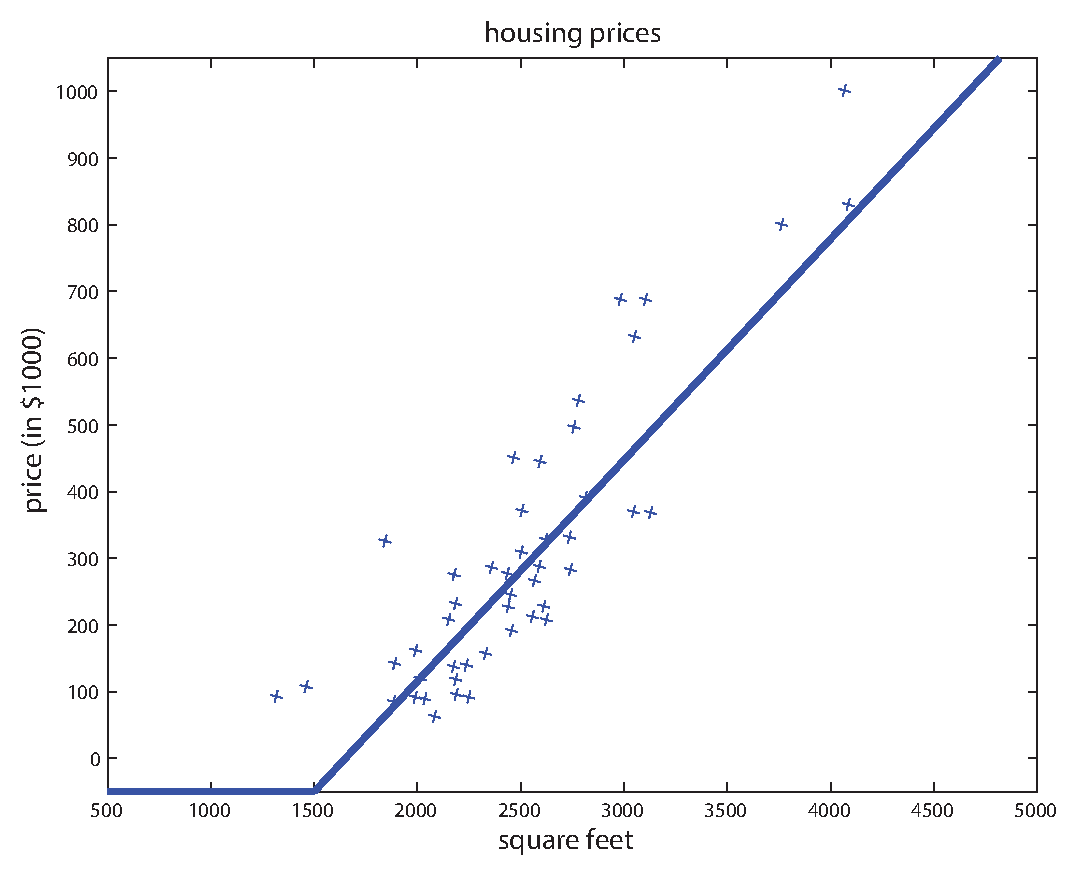
\includegraphics[width=0.6\linewidth]{housingDataReLU.eps}
	\caption{Housing prices with a ``kink" in the graph.}\label{fig:housing}
\end{figure}

Given these features (size, number of bedrooms, zip code, and wealth), we might then decide that the price of the house depends on the maximum family size it can accommodate. Suppose the family size is a function of the size of the house and number of bedrooms (see Figure \ref{fig:mininet}). The zip code may provide additional information such as how walkable the neighborhood is (i.e., can you walk to the grocery store or do you need to drive everywhere). Combining the zip code with the wealth of the neighborhood may predict the quality of the local elementary school. Given these three derived features (family size, walkable, school quality), we may conclude that the price of the home ultimately depends on these three features.

\begin{figure}[h]
	\centering
	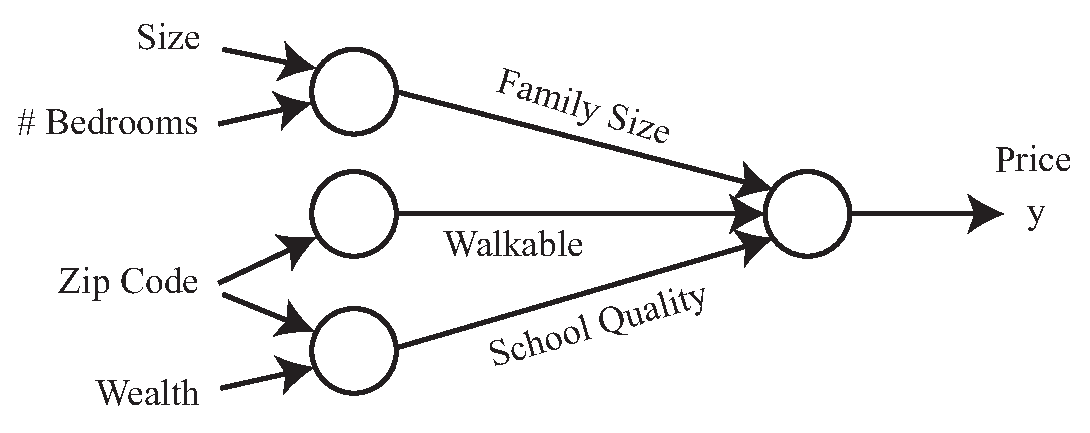
\includegraphics[width=0.6\linewidth]{mini_net.eps}
	\caption{Diagram of a small neural network for predicting housing prices.}\label{fig:mininet}
\end{figure}

We have described this neural network as if you (the reader) already have the insight to determine these three factors ultimately affect the housing price. Part of the magic of a neural network is that all you need are the input features $x$ and the output $y$ while the neural network will figure out everything in the middle by itself.
The process of a neural network learning the intermediate features is called \textit{end-to-end learning}.

Following the housing example, formally, the input to a neural network is a set of input features $x_1, x_2, x_3, x_4$. We connect these four features to three neurons. These three "internal" neurons are called \textit{hidden units}. The goal for the neural network is to automatically determine three relevant features such that the three features predict the price of a house. The only thing we must provide to the neural network is a sufficient number of training examples $(x^{(i)}, y^{(i)})$. Often times, the neural network will discover complex features which are very useful for predicting the output but may be difficult for a human to understand since it does not have a ``common" meaning. This is why some people refer to neural networks as a \textit{black box}, as it can be difficult to understand the features it has invented.

Let us formalize this neural network representation. Suppose we have three input features $x_1, x_2, x_3$ which are collectively called the \textit{input layer}, four hidden units which are collectively called the \textit{hidden layer} and one output neuron called the \textit{output layer}. The term hidden layer is called ``hidden" because we do not have the ground truth/training value for the hidden units. This is in contrast to the input and output layers, both of which we know the ground truth values from $(x^{(i)}, y^{(i)})$.

The first hidden unit requires the input $x_1, x_2, x_3$ and outputs a value denoted by $a_1$. We use the letter $a$ since it refers to the neuron's ``activation" value. In this particular example, we have a single hidden layer but it is possible to have multiple hidden layers. Let $a_1^{[1]}$ denote the output value of the first hidden unit in the first hidden layer. We use zero-indexing to refer to the layer numbers. That is, the input layer is layer 0, the first hidden layer is layer 1 and the output layer is layer 2. Again, more complex neural networks may have more hidden layers. Given this mathematical notation, the output of layer 2 is $a^{[2]}_1$. We can unify our notation:
\begin{align}
x_1 &= a^{[0]}_1 \\
x_2 &= a^{[0]}_2 \\
x_3 &= a^{[0]}_3
\end{align}
To clarify, $\textrm{foo}^{[1]}$ with brackets denotes anything associated with layer 1, $x^{(i)}$ with parenthesis refers to the $i^{th}$ training example, and $a^{[\ell]}_j$ refers to the activation of the $j^{th}$ unit in layer $\ell$. If we look at logistic regression $g(x)$ as a single neuron (see Figure \ref{fig:single}):

\begin{equation*}
g(x) = \frac{1}{1+\exp(-(w^Tx+b))}
\end{equation*}
The input to the logistic regression $g(x)$ is three features $x_1, x_2$ and $x_3$ and it outputs an estimated value of $y$. We can represent $g(x)$ with a single neuron in the neural network. We can break $g(x)$ into two distinct computations: (1) $z= w^T x + b $ and (2) $a = \sigma(z)$ where $\sigma(z) = 1/(1+e^{-z})$. Note the notational difference: previously we used $z=\theta^T x$ but now we are using $z=w^T x + b$, where $w$ is a vector. Later in these notes you will see capital $W$ to denote a matrix. The reasoning for this notational difference is conform with standard neural network notation. More generally, $a= g(z)$ where $g(z)$ is some activation function. Example activation functions include:
\begin{align}
g(z) &= \frac{1}{1+e^{-z}} \textrm{\qquad (sigmoid)} \\
g(z) &= \max(z, 0) \textrm{\qquad (ReLU)} \\
g(z) &= \frac{e^z-e^{-z}}{e^z + e^{-z}} \textrm{\qquad (tanh)}
\end{align}
In general, $g(z)$ is a non-linear function.
\begin{figure}[h]
	\centering
	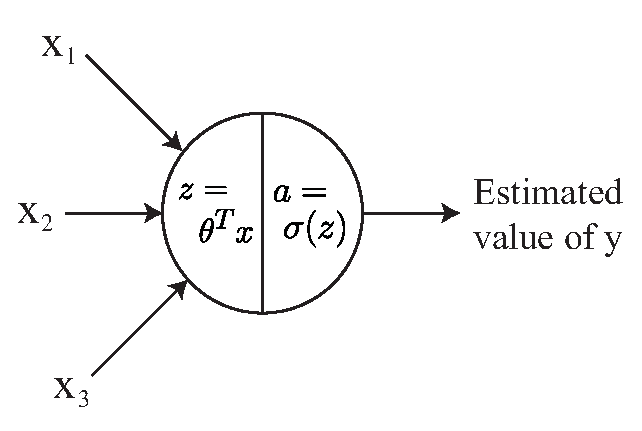
\includegraphics[width=0.5\linewidth]{single_neuron.eps}
	\caption{Logistic regression as a single neuron.}\label{fig:single}
\end{figure}

\noindent Returning to our neural network from before, the first hidden unit in the first hidden layer will perform the following computation:
\begin{equation}
z_1^{[1]} = {W^{[1]}_1}^T x + b^{[1]}_1 \quad\textrm{and}\quad a_1^{[1]} = g(z_1^{[1]})
\end{equation}
where $W$ is a matrix of parameters and $W_1$ refers to the first row of this matrix.  
The parameters associated with the first hidden unit is the vector $W^{[1]}_1 \in \mathbb{R}^3$ and the scalar $b^{[1]}_1 \in \mathbb{R}$. For the second and third hidden units in the first hidden layer, the computation is defined as:
\begin{align*}
z_2^{[1]} = {W^{[1]}_2}^T x + b^{[1]}_2 \quad\textrm{and}\quad a_2^{[1]} = g(z_2^{[1]}) \\
z_3^{[1]} = {W^{[1]}_3}^T x + b^{[1]}_3 \quad\textrm{and}\quad a_3^{[1]} = g(z_3^{[1]})
\end{align*}
where each hidden unit has its corresponding parameters $W$ and $b$. Moving on, the output layer performs the computation:
\begin{align}
z_1^{[2]} = {W^{[2]}_1}^T a^{[1]} + b^{[2]}_1 \quad\textrm{and}\quad a_1^{[2]} = g(z_1^{[2]})
\end{align}
where $a^{[1]}$ is defined as the concatenation of all first layer activations:
\begin{equation}
a^{[1]} = \left[ \begin{array}{c}
a^{[1]}_1 \\
a^{[1]}_2 \\
a^{[1]}_3 \\
a^{[1]}_4
\end{array}\right]
\end{equation}
The activation $a_1^{[2]}$ from the second layer, which is a single scalar as defined by $a_1^{[2]}=g(z_1^{[2]})$, represents the neural network's final output prediction. Note that for regression tasks, one typically does not apply a non-linear function which is strictly positive (i.e., ReLU or sigmoid) because for some tasks, the ground truth $y$ value may in fact be negative.

\section{Vectorization}

In order to implement a neural network at a reasonable speed, one must be careful when using for loops. In order to compute the hidden unit activations in the first layer, we must compute $z_1, ..., z_4$ and $a_1,..., a_4$.
\begin{align}
z_1^{[1]} & = {W^{[1]}_1}^T x + b^{[1]}_1 \quad\textrm{and}\quad a_1^{[1]} = g(z_1^{[1]}) \\
& \vdots \qquad \qquad \qquad \qquad \vdots \qquad \qquad \qquad \vdots \\
z_4^{[1]} & = {W^{[1]}_4}^T x + b^{[1]}_4 \quad\textrm{and}\quad a_4^{[1]} = g(z_4^{[1]})
\end{align}
The most natural way to implement this in code is to use a for loop. One of the treasures that deep learning has given to the field of machine learning is that deep learning algorithms have high computational requirements. As a result, code will run very slowly if you use for loops.

This gave rise to \textit{vectorization}. Instead of using for loops, vectorization takes advantage of matrix algebra and highly optimized numerical linear algebra packages (e.g., BLAS) to make neural network computations run quickly. Before the deep learning era, a for loop may have been sufficient on smaller datasets, but modern deep networks and state-of-the-art datasets will be infeasible to run with for loops.

\subsection{Vectorizing the Output Computation}

We now present a method for computing $z_1,...,z_4$ without a for loop. Using our matrix algebra, we can compute the activations:
\begin{equation}\label{eq:z1}
\underbrace{
\left[\begin{array}{c}
z^{[1]}_1 \\
\vdots \\
\vdots \\
z^{[1]}_4
\end{array} \right]}_{\mbox{\normalsize $z^{[1]} \in \mathbb{R}^{4\times 1}$}}
= \;\;
\underbrace{
\left[ \begin{tabular}{c}
--- ${W^{[1]}_1}^T$ --- \\
--- ${W^{[1]}_2}^T$ --- \\
\vdots \\ 
--- ${W^{[1]}_4}^T$ --- 
\end{tabular}\right]}_{\mbox{\normalsize $W^{[1]} \in \mathbb{R}^{4\times 3}$}}
\;
\underbrace{
\left[\begin{array}{c}
x_1 \\
x_2 \\
x_3
\end{array}
\right]}_{\mbox{\normalsize $x \in \mathbb{R}^{3\times 1}$}} + 
\underbrace{
\left[\begin{array}{c}
b^{[1]}_1 \\
b^{[1]}_2 \\
\vdots \\
b^{[1]}_4
\end{array} \right]
}_{\mbox{\normalsize $b^{[1]} \in \mathbb{R}^{4\times 1}$}}
\end{equation}
Where the $\mathbb{R}^{\di \times \nexp}$ beneath each matrix indicates the dimensions. Expressing this in matrix  notation: $z^{[1]} = W^{[1]} x + b^{[1]}$. To compute $a^{[1]}$ without a for loop, we can leverage vectorized libraries in Matlab, Octave, or Python which compute $a^{[1]} = g(z^{[1]})$ very fast by performing parallel element-wise operations. Mathematically, we defined the sigmoid function $g(z)$ as:
\begin{equation}
g(z) = \frac{1}{1+e^{-z}} \qquad \textrm{ where } z \in \mathbb{R}
\end{equation}
\noindent However, the sigmoid function can be defined not only for scalars but also vectors. In a Matlab/Octave-like pseudocode, we can define the sigmoid as:
\begin{equation}
g(z) = \texttt{1 ./ (1+exp(-}z\texttt{))}\qquad \textrm{ where } z \in \mathbb{R}^\di
\end{equation}
where \texttt{./} denotes element-wise division. With this vectorized implementation, $a^{[1]} = g(z^{[1]})$ can be computed quickly.

To summarize the neural network so far, given an input $x \in \mathbb{R}^3$, we compute the hidden layer's activations with $z^{[1]} = W^{[1]} x + b^{[1]}$ and $a^{[1]} = g(z^{[1]})$. To compute the output layer's activations (i.e., neural network output):
\begin{equation}\label{eq:z2}
\underbrace{ z^{[2]} }_{1\times 1} = \underbrace{ W^{[2]} }_{1\times 4} \underbrace{ a^{[1]} }_{4\times 1} + \underbrace{ b^{[2]} }_{1\times 1} \quad \textrm{ and } \quad \underbrace{ a^{[2]} }_{1\times 1} = g(\underbrace{ z^{[2]} }_{1\times 1} )
\end{equation}

Why do we not use the identity function for $g(z)$? That is, why not use $g(z) = z$? Assume for sake of argument that $b^{[1]}$ and $b^{[2]}$ are zeros. Using Equation (\ref{eq:z2}), we have:
\begin{align}
z^{[2]} &= W^{[2]} a^{[1]} \\
&= W^{[2]} g(z^{[1]}) && \text{by definition}\\
&= W^{[2]} z^{[1]} && \text{since $g(z) = z$} \\
&= W^{[2]} W^{[1]} x && \text{from Equation (\ref{eq:z1})} \\
&= \tilde{W} x && \text{where $\tilde{W} = W^{[2]} W^{[1]}$ }
\end{align}
Notice how $W^{[2]} W^{[1]}$ collapsed into $\tilde{W}$.
This is because applying a linear function to another linear function will result in a linear function over the original input (i.e., you can construct a $\tilde{W}$ such that $\tilde{W}x = W^{[2]} W^{[1]} x$). This loses much of the representational power of the neural network as often times the output we are trying to predict has a non-linear relationship with the inputs. Without non-linear activation functions, the neural network will simply perform linear regression.

\subsection{Vectorization Over Training Examples}

Suppose you have a training set with three examples. The activations for each example are as follows:
\begin{align*}
z^{[1](1)} = W^{[1]} x^{(1)} + b^{[1]} \\
z^{[1](2)} = W^{[1]} x^{(2)} + b^{[1]} \\
z^{[1](3)} = W^{[1]} x^{(3)} + b^{[1]}
\end{align*}
Note the difference between square brackets $[\cdot]$, which refer to the layer number, and parenthesis $(\cdot)$, which refer to the training example number. Intuitively, one would implement this using a for loop. It turns out, we can vectorize these operations as well. First, define:
\begin{equation}
X = \left[\begin{array}{ccc}
| & | & | \\
x^{(1)} & x^{(2)} & x^{(3)} \\
| & | & |
\end{array} \right]
\end{equation}
Note that we are stacking training examples in columns and \textit{not} rows. We can then combine this into a single unified formulation:
\begin{equation}\label{eq:concat}
Z^{[1]} = \left[\begin{array}{ccc}
| & | & | \\
z^{[1](1)} & z^{[1](2)} & z^{[1](3)} \\
| & | & |
\end{array} \right] = W^{[1]} X + b^{[1]}
\end{equation}
You may notice that we are attempting to add $b^{[1]} \in \mathbb{R}^{4 \times 1}$ to $W^{[1]} X \in \mathbb{R}^{4 \times 3}$. Strictly following the rules of linear algebra, this is not allowed.
In practice however, this addition is performed using \textit{broadcasting}.
We create an intermediate $\tilde{b}^{[1]} \in \mathbb{R}^{4 \times 3}$:
\begin{equation}
\tilde{b}^{[1]} = \left[\begin{array}{ccc}
| & | & | \\
b^{[1]} & b^{[1]} & b^{[1]} \\
| & | & |
\end{array} \right]
\end{equation}
We can then perform the computation: $Z^{[1]}  = W^{[1]} X + \tilde{b}^{[1]}$.
Often times, it is not necessary to explicitly construct $\tilde{b}^{[1]}$. By inspecting the dimensions in (\ref{eq:concat}), you can assume $b^{[1]} \in \mathbb{R}^{4 \times 1}$ is correctly broadcast to $W^{[1]} X \in \mathbb{R}^{4 \times 3}$.

Putting it together: Suppose we have a training set $(x^{(1)},y^{(1)}), ..., (x^{(\nexp)}, y^{(\nexp)})$ where $x^{(i)}$ is a picture and $y^{(i)}$ is a binary label for whether the picture contains a cat or not (i.e., 1=contains a cat). First, we initialize the parameters $W^{[1]}, b^{[1]}, W^{[2]}, b^{[2]}$ to small random numbers. For each example, we compute the output ``probability" from the sigmoid function $a^{[2](i)}$. Second, using the logistic regression log likelihood:
\begin{equation}
	\sum\limits_{i=1}^{\nexp} \Big( y^{(i)}\log a^{[2](i)} + (1-y^{(i)}) \log (1-a^{[2](i)})\Big)
\end{equation}
Finally, we maximize this function using gradient ascent. This maximization procedure corresponds to training the neural network.

\section{Backpropagation}

Instead of the housing example, we now have a new problem. Suppose we wish to detect whether there is a soccer ball in an image or not. Given an input image $x^{(i)}$, we wish to output a binary prediction 1 if there is a ball in the image and 0 otherwise.

Aside: Images can be represented as a matrix with number of elements equal to the number of pixels. However, color images are digitally represented as a volume (i.e., three-channels; or three matrices stacked on each other). The number three is used because colors are represented as red-green-blue (RGB) values. In the diagram below, we have a $64 \times 64 \times 3$ image containing a soccer ball. It is \textit{flattened} into a single vector containing 12,288 elements.

\begin{figure}[h]
	\centering
	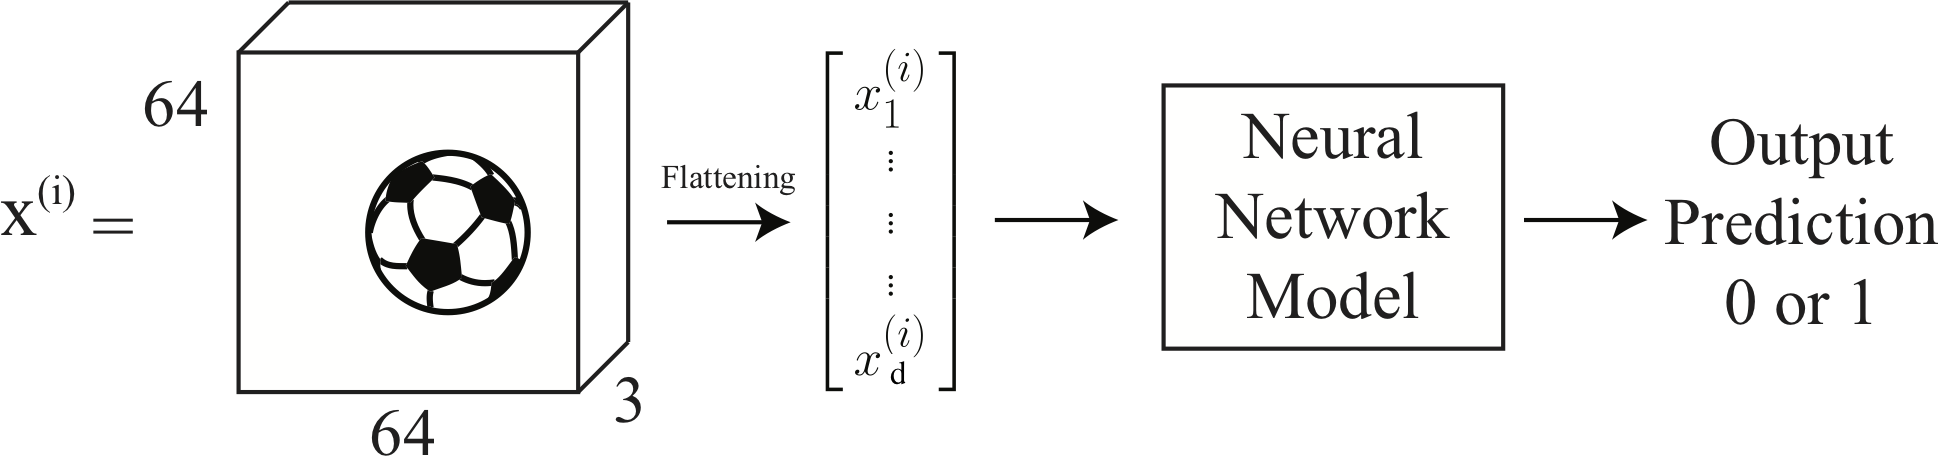
\includegraphics[width=0.90\linewidth]{image_d}
\end{figure}

A neural network \textit{model} consists of two components: (i) the network architecture, which defines how many layers, how many neurons, and how the neurons are connected and (ii) the parameters (values; also known as weights).
In this section, we will talk about how to learn the parameters. First we will talk about parameter initialization, optimization and analyzing these parameters.

\subsection{Parameter Initialization}

Consider a two layer neural network. On the left, the input is a flattened image vector $x^{(i)}_{1}, ..., x^{(i)}_{\di}$. In the first hidden layer, notice how all inputs are connected to all neurons in the next layer. This is called a \textit{fully connected} layer.
\begin{center}
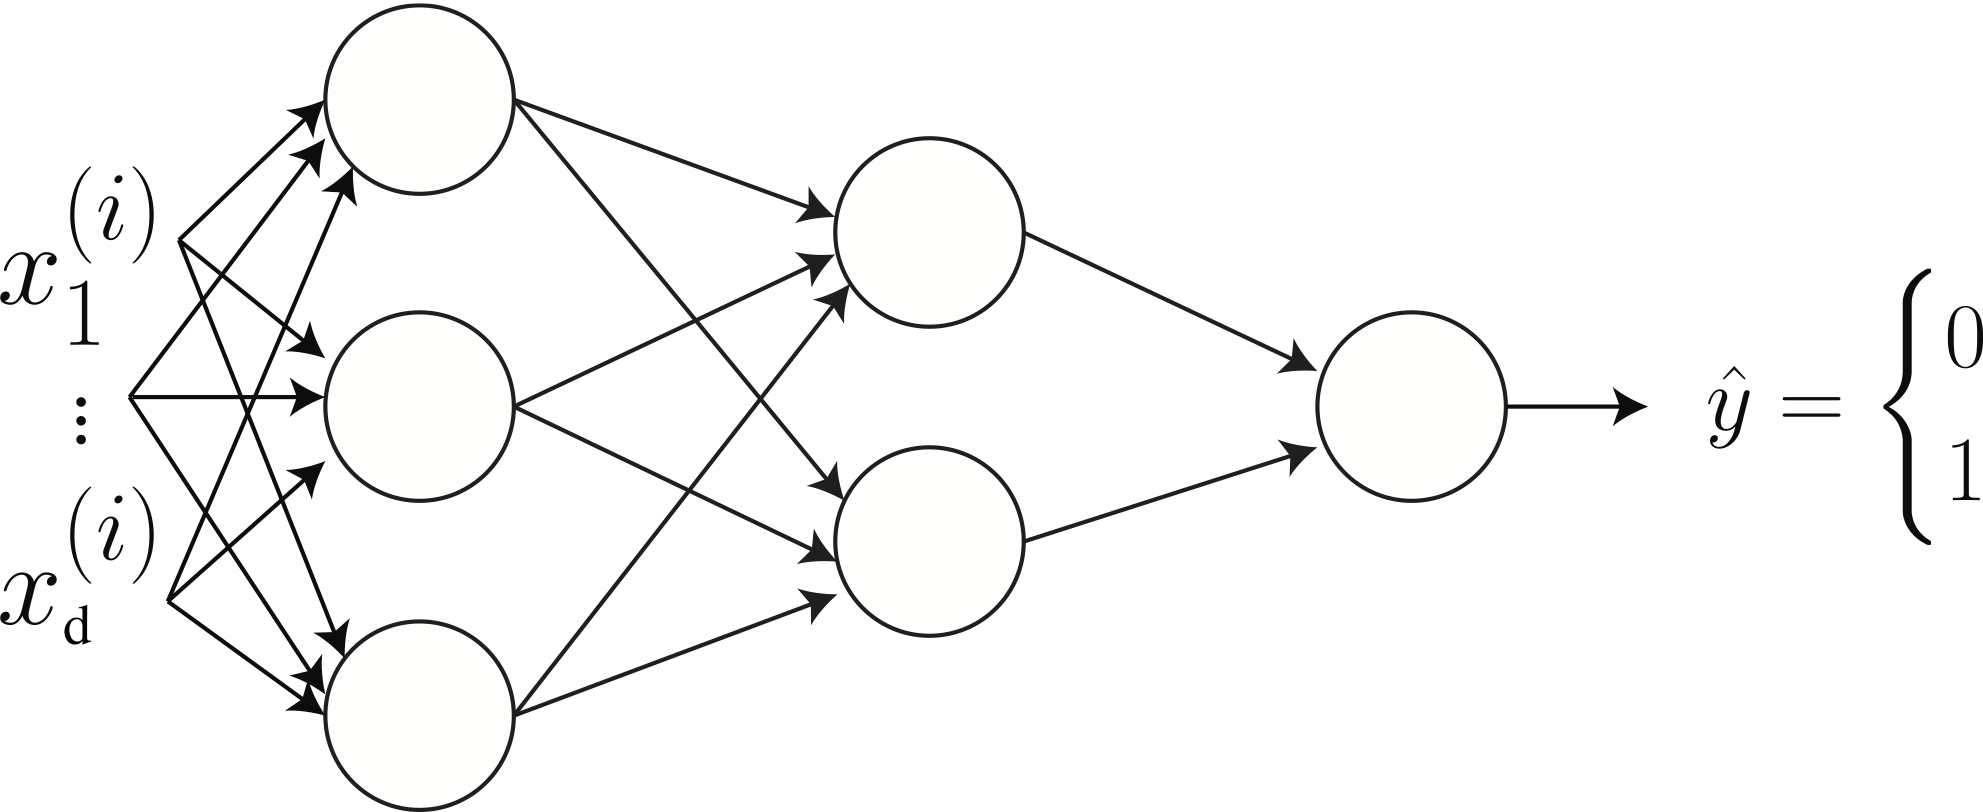
\includegraphics[width=0.80\linewidth]{two_layer_d}\\
\end{center}
The next step is to compute how many parameters are in this network. One way of doing this is to compute the forward propagation by hand.
\begin{align}
z^{[1]} &= W^{[1]} x^{(i)} + b^{[1]} \\
a^{[1]} &= g(z^{[1]}) \\
z^{[2]} &= W^{[2]} a^{[1]} + b^{[2]} \\
a^{[2]} &= g(z^{[2]}) \\ \label{eq:a2}
z^{[3]} &= W^{[3]} a^{[2]} + b^{[3]} \\ \label{eq:z3}
\hat{y}^{(i)} &= a^{[3]} = g(z^{[3]})
\end{align}
We know that $z^{[1]}, a^{[1]}\in \mathbb{R}^{3\times 1} $ and $z^{[2]}, a^{[2]}\in \mathbb{R}^{2\times 1} $  and  $z^{[3]}, a^{[3]}\in \mathbb{R}^{1 \times 1} $.
As of now, we do not know the size of $W^{[1]}$.
However, we can compute its size. We know that $x \in \mathbb{R}^{\di \times 1}$.
This leads us to the following
\begin{equation}
z^{[1]} = W^{[1]} x^{(i)} \in \mathbb{R}^{3 \times 1} \textrm{\quad Written as sizes: \quad} \mathbb{R}^{3 \times 1} = \mathbb{R}^{? \times ?} \times  \mathbb{R}^{\di \times 1}
\end{equation}
Using matrix multiplication, we conclude that $? \times ?$ must be $3 \times \di$. We also conclude that the bias is of size $3 \times 1$ because its size must match $W^{[1]} x^{(i)}$. 
We repeat this process for each hidden layer.
This gives us:
\begin{equation}
W^{[2]} \in \mathbb{R}^{2 \times 3}, b^{[2]} \in \mathbb{R}^{2 \times 1} \textrm{\quad and \quad} W^{[3]} \in \mathbb{R}^{1 \times 2}, b^{[3]} \in \mathbb{R}^{1 \times 1}
\end{equation}
In total, we have $3\di+3$ in the first layer, $2\times3 + 2$ in the second layer and $2 + 1$ in the third layer. This gives us a total of $3\di + 14$ parameters.

Before we start training the neural network, we must select an initial value for these parameters.
We do not use the value zero as the initial value.
This is because the output of the first layer will always be the same since $  W^{[1]} x^{(i)} + b^{[1]} = 0^{3 \times d} x^{(i)} + 0^{3 \times 1}$ where $0^{\nexp \times \di}$ denotes a matrix of size $\nexp \times \di$ filled with zeros.
This will cause problems later on when we try to update these parameters (i.e., the gradients will all be the same).
The solution is to randomly initialize the parameters to small values (e.g., normally distributed around zero; $\mathcal{N}(0, 0.1))$.
Once the parameters have been initialized, we can begin training the neural network with gradient descent.

The next step of the training process is to update the parameters.
After a single forward pass through the neural network, the output will be a predicted value $\hat{y}$.
We can then compute the loss $\mathcal{L}$, in our case the log loss:
\begin{equation}
\mathcal{L}(\hat{y}, y) = -\bigg[(1-y) \log(1 - \hat{y}) + y \log \hat{y}\bigg]
\end{equation}
The loss function $\mathcal{L}(\hat{y}, y)$ produces a single scalar value. For short, we will refer to the loss value as $\mathcal{L}$.
Given this value, we now must update all parameters in layers of the neural network.
For any given layer index $\ell$, we update them:
\begin{align}\label{eq:dW}
W^{[\ell]} &= W^{[\ell]} - \alpha \frac{\partial \mathcal{L}}{\partial W^{[\ell]}} \\ \label{eq:db}
b^{[\ell]} &= b^{[\ell]} - \alpha \frac{\partial \mathcal{L}}{\partial b^{[\ell]}}
\end{align}
where $\alpha$ is the learning rate. To proceed, we must compute the gradient with respect to the parameters: $\partial \mathcal{L}/\partial W^{[\ell]}$ and $\partial \mathcal{L} / \partial b^{[\ell]}$.

Remember, we made a decision to not set all parameters to zero.
What if we had initialized all parameters to be zero?
We know that $z^{[3]} = W^{[3]} a^{[2]} + b^{[3]}$ will evaluate to zero, because $W^{[3]}$ and $b^{[3]}$ are all zero.
However, the output of the neural network is defined as $a^{[3]} = g(z^{[3]})$.
Recall that $g(\cdot)$ is defined as the sigmoid function. This means $a^{[3]}=  g(0)=0.5$.
Thus, no matter what value of $x^{(i)}$ we provide, the network will output $\hat{y} = 0.5$.

What if we had initialized all parameters to be the same non-zero value?
In this case, consider the activations of the first layer:
\begin{equation}
a^{[1]} = g(z^{[1]}) = g(W^{[1]} x^{(i)} + b^{[1]})
\end{equation}
Each element of the activation vector $a^{[1]}$ will be the same (because $W^{[1]}$ contains all the same values).
This behavior will occur at all layers of the neural network.
As a result, when we compute the gradient, all neurons in a layer will be equally responsible for anything contributed to the final loss.
We call this property \textit{symmetry}.
This means each neuron (within a layer) will receive the exact same gradient update value (i.e., all neurons will learn the same thing).

In practice, it turns out there is something better than random initialization.
It is called Xavier/He initialization and initializes the weights:
\begin{equation}
w^{[\ell]} \sim \mathcal{N}\left(0,  \sqrt{ \frac{2}{n^{[\ell]} + n^{[\ell - 1]} }} \right)
\end{equation}
where $n^{[\ell]}$ is the number of neurons in layer $\ell$. This acts as a mini-normalization technique. For a single layer, consider the variance of the input to the layer as $\sigma^{(in)}$ and the variance of the output (i.e., activations) of a layer to be $\sigma^{(out)}$. Xavier/He initialization encourages $\sigma^{(in)}$ to be similar to $\sigma^{(out)}$. 

\subsection{Optimization}
 
Recall our neural network parameters: $W^{[1]}, b^{[1]}, W^{[2]}, b^{[2]}, W^{[3]}, b^{[3]}$.
To update them, we use stochastic gradient descent (SGD) using the update rules in Equations (\ref{eq:dW}) and (\ref{eq:db}). So our goal is to calculate $\frac{\partial \mathcal{L}}{\partial W^{[1]}}$, $\frac{\partial \mathcal{L}}{\partial W^{[2]}}$, $\frac{\partial \mathcal{L}}{\partial W^{[3]}}$, $\frac{\partial \mathcal{L}}{\partial b^{[1]}}$, $\frac{\partial \mathcal{L}}{\partial b^{[2]}}$ and $\frac{\partial \mathcal{L}}{\partial b^{[3]}}$. In what follows we will compute the gradient with respect to $W^{[2]}$ and leave the rest as an exercise since they are very similar.

First, observe that
\begin{align*}
\frac{\partial \mathcal{L}}{\partial W^{[2]}} &= \begin{bmatrix} \frac{\partial \mathcal{L}}{\partial W^{[2]}_{11}} & \frac{\partial \mathcal{L}}{\partial W^{[2]}_{12}} & \frac{\partial \mathcal{L}}{\partial W^{[2]}_{13}} \\
\frac{\partial \mathcal{L}}{\partial W^{[2]}_{21}} & \frac{\partial \mathcal{L}}{\partial W^{[2]}_{22}} & \frac{\partial \mathcal{L}}{\partial W^{[2]}_{23}} \end{bmatrix},
\end{align*}
and also observe that
\begin{align*}
\frac{\partial \mathcal{L}}{\partial z^{[3]}} &= \frac{\partial}{\partial z^{[3]}}\left[-y\log \hat{y} - (1-y)\log (1-\hat{y})\right] \\
&= \frac{\partial}{\partial z^{[3]}}\left[-y\log \sigma(z^{[3]}) - (1-y)\log (1-\sigma(z^{[3]}))\right] \quad \text{ (where $\sigma$ is the sigmoid function)}\\
&= -y\frac{1}{\sigma(z^{[3]})}\sigma(z^{[3]})(1-\sigma(z^{[3]})) - (1-y)\frac{1}{(1-\sigma(z^{[3]}))}(-1)\sigma(z^{[3]})(1-\sigma(z^{[3]})) \\
&= -y(1-\sigma(z^{[3]}) + (1-y)\sigma(z^{[3]}) \\
&= \sigma(z^{[3]}) - y \\
&= a^{[3]} - y.
\end{align*}

Now to calculate the gradient w.r.t $\frac{\partial \mathcal{L}}{\partial W^{[2]}_{ij}}$, we use the multivariate chain rule of calculus:
\begin{align*}
\frac{\partial \mathcal{L}}{\partial W^{[2]}_{ij}} &= \frac{\partial \mathcal{L}}{\partial \hat{y}} \frac{\partial \hat{y}}{\partial W^{[2]}_{ij}} \\
&= \frac{\partial \mathcal{L}}{\partial a^{[3]}} \frac{\partial a^{[3]}}{\partial W^{[2]}_{ij}} \\
&= \frac{\partial \mathcal{L}}{\partial a^{[3]}} \frac{\partial a^{[3]}}{\partial z^{[3]}} \frac{\partial z^{[3]}}{\partial W^{[2]}_{ij}} \\
&= \frac{\partial \mathcal{L}}{\partial a^{[3]}} \frac{\partial a^{[3]}}{\partial z^{[3]}} \frac{\partial z^{[3]}}{\partial a^{[2]}} \frac{\partial a^{[2]}}{\partial W^{[2]}_{ij}} \\
&= \underbrace{\frac{\partial \mathcal{L}}{\partial a^{[3]}}  \frac{\partial a^{[3]}}{\partial z^{[3]}} }_{ \underbrace{(a^{[3]}-y)}_{1\times 1} } \quad \underbrace{ \frac{\partial z^{[3]}}{\partial a^{[2]}} }_{ \underbrace{ W^{[3]} }_{1\times 2} } \quad \underbrace{ \frac{\partial a^{[2]}}{\partial z^{[2]}} }_{ \underbrace{\text{diag} \left(g'(z^{[2]})\right)  }_{2\times 2} } \quad \underbrace{\frac{\partial z^{[2]}} {\partial W^{[2]}_{ij}}}_{\underbrace{a^{[1]}_j\mathbf{e_i} }_{2\times 1} } \\
&\quad\text{(where $a^{[1]} \in \mathbb{R}^3$, and $\mathbf{e_i} \in \mathbb{R}^2$ is the $i^{th}$ basis vector)} \\
&= \underbrace{ (a^{[3]}-y) W^{[3]} \circ g'(z^{[2]}) }_{1\times 2} \quad \underbrace{a^{[1]}_j\mathbf{e_i} }_{2\times 1}  \\
&= \underbrace{ \left[(a^{[3]}-y) W^{[3]} \circ g'(z^{[2]})\right]_i a^{[1]}_j }_{1\times 1} \\
\Rightarrow \frac{\partial \mathcal{L}}{\partial W^{[2]}} &= \underbrace{ \left[(a^{[3]}-y) W^{[3]} \circ g'(z^{[2]})\right]^T {a^{[1]^T}}}_{2\times 3}
\end{align*}
where $\circ$ indicates elementwise product (Hadamard product). We leave the remaining gradients as an exercise to the reader.

Returning to optimization, we previously discussed stochastic gradient descent. Now we will talk about gradient descent.
For any single layer $\ell$, the update rule is defined as:
\begin{equation}
W^{[\ell]} = W^{[\ell]} - \alpha \frac{\partial J}{\partial W^{[\ell]}}
\end{equation}
where $J$ is the cost function $J = \frac{1}{\nexp} \sum\limits_{i=1}^{\nexp} \mathcal{L}^{(i)}$ and $\mathcal{L}^{(i)}$ is the loss for a single example.
The difference between the gradient descent update versus the stochastic gradient descent version is that the cost function $J$ gives more accurate gradients whereas $\mathcal{L}^{(i)}$ may be noisy.
Stochastic gradient descent attempts to approximate the gradient from (full) gradient descent.
The disadvantage of gradient descent is that it can be difficult to compute all activations for all examples in a single forward or backwards propagation phase.

In practice, research and applications use \textit{mini-batch gradient descent}. This is a compromise between gradient descent and stochastic gradient descent. In the case mini-batch gradient descent, the cost function $J_{\textrm{mb}}$ is defined as follows:
\begin{equation}
J_{\textrm{mb}} = \frac{1}{\textrm{B}} \sum\limits_{i=1}^{\textrm{B}} \mathcal{L}^{(i)}
\end{equation}
where $B$ is the number of examples in the mini-batch.

There is another optimization method called \textit{momentum}. Consider mini-batch stochastic gradient. For any single layer $\ell$, the update rule is as follows:
\begin{align}
\begin{cases}
v_{dW^{[\ell]}} = \beta v_{dW^{[\ell]}} + (1- \beta) \frac{\partial J}{\partial W^{[\ell]}} \\
W^{[\ell]} =  W^{[\ell]} - \alpha v_{dW^{[\ell]}}
\end{cases}
\end{align}
Notice how there are now two stages instead of a single stage. The weight update now depends on the cost $J$ at this update step and the \textit{velocity} $v_{dW^{[\ell]}}$. The relative importance is controlled by $\beta$.
Consider the analogy to a human driving a car. While in motion, the car has momentum.
If the car were to use the brakes (or not push accelerator throttle), the car would continue moving due to its momentum.
Returning to optimization, the velocity $v_{dW^{[\ell]}}$ will keep track of the gradient over time.
This technique has significantly helped neural networks during the training phase.

\subsection{Analyzing the Parameters}

At this point, we have initialized the parameters and have optimized the parameters.
Suppose we evaluate the trained model and observe that it achieves 96\% accuracy on the training set but only 64\% on the testing set.
Some solutions include: collecting more data, employing regularization, or making the model shallower.
Let us briefly look at regularization techniques.

\subsubsection{L2 Regularization}

Let $W$ below denote \textit{all} the parameters in a model. In the case of neural networks, you may think of applying the 2nd term to all layer weights $W^{[\ell]}$. For convenience, we simply write $W$. The L2 regularization adds another term to the cost function:
\begin{align}\label{eq:l2_1}
J_{L2} &= J + \frac{\lambda}{2} ||W||^2 \\ \label{eq:l2_2}
	   &= J + \frac{\lambda}{2} \sum\limits_{ij} | W_{ij} |^2 \\ \label{eq:l2_3}
	   &= J + \frac{\lambda}{2} W^T W 
\end{align}
where $J$ is the standard cost function from before, $\lambda$ is an arbitrary value with a larger value indicating more regularization and $W$ contains all the weight matrices, and where Equations (\ref{eq:l2_1}), (\ref{eq:l2_2}) and (\ref{eq:l2_3}) are equivalent. The update rule with L2 regularization becomes:
\begin{align}
W &= W - \alpha \frac{\partial J}{\partial W} - \alpha \frac{\lambda}{2} \frac{\partial W^T W}{\partial W} \\
&= (1 - \alpha \lambda) W - \alpha \frac{\partial J}{\partial W}
\end{align}
When we were updating our parameters using gradient descent, we did not have the $(1 - \alpha \lambda)W$ term.
This means with L2 regularization, every update will include some penalization, depending on $W$.
This penalization increases the cost $J$, which encourages individual parameters to be small in magnitude, which is a way to reduce overfitting.

\subsubsection{Parameter Sharing}

Recall logistic regression. It can be represented as a neural network, as shown in Figure \ref{fig:single}.
The parameter vector $\theta = (\theta_1, ..., \theta_{\di})$ must have the same number of elements as the input vector $x = (x_1, ..., x_{\di})$. In our image soccer ball example, this means $\theta_1$ always looks at the top left pixel of the image no matter what.
However, we know that a soccer ball might appear in any region of the image and not always the center.
It is possible that $\theta_1$ was never trained on a soccer ball in the top left of the image.
As a result, during test time, if an image of a soccer ball in the top left appears, the logistic regression will likely predict \textit{no soccer ball}. This is a problem.

This leads us to \textit{convolutional neural networks}. Suppose $\theta$ is no longer a vector but instead is a matrix.
For our soccer ball example, suppose $\theta = \mathbb{R}^{4 \times 4}$.
\begin{figure}[h]
\centering
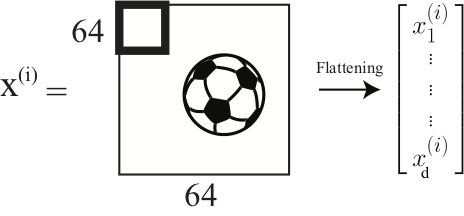
\includegraphics[width=0.6\linewidth]{cnn_d}
\end{figure}
For simplicity, we show the image as $64 \times 64$ but recall it is actually three-dimensional and contains 3 channels. 
We now take our matrix of parameters $\theta$ and slide it over the image. This is shown above by the thick square in the upper left of the image.
To compute the activation $a$, we compute the element-wise product between $\theta$ and $x_{1:4,1:4}$, where the subscripts for $x$ indicate we are taking the top left $4 \times 4$ region in the image $x$.
We then collapse the matrix into a single scalar by summing all the elements resulting from the element-wise product. Formally:
\begin{equation}
a = \sum\limits_{i=1}^{4} \sum\limits_{j=1}^{4} \theta_{ij} x_{ij}
\end{equation}
We then move this window slightly to the right in the image and repeat this process. Once we have reached the end of the row, we start at the beginning of the second row.
\begin{center}
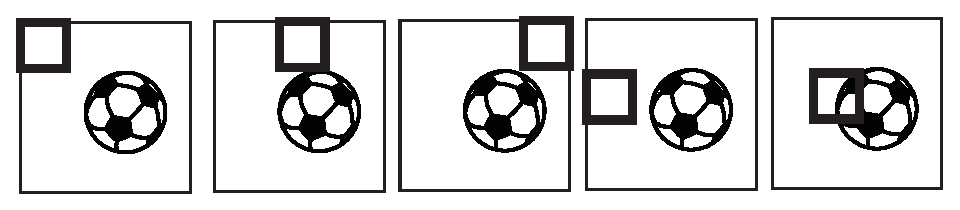
\includegraphics[width=0.9\linewidth]{sliding_window.eps}
\end{center}
Once we have reached the end of the image, the parameters $\theta$ have ``seen" all pixels of the image: $\theta_1$ is no longer related to only the top left pixel.
As a result, whether the soccer ball appears in the bottom right or top left of the image, the neural network will successfully detect the soccer ball.\blfootnote{Last Updated: \today}

\end{document}


